\textbf{Prime Number Theorem}
\begin{enumerate}
\item $\sum_{n=1}^\infty\frac{\mu(n)}{n}=0$
\item $\sum_{n\leq x}\mu(n)=o(x)$
\item $\psi(x)\sim x$
\item $\vartheta(x)\sim x$
\item $\pi(x)\sim\frac{x}{\log x}$
\item $p(n)\sim n\log n$
\end{enumerate}
\textbf{$(2)\implies(3)$} \\
MST
\begin{align*}
\frac1x\psi(x) &\to 1 \\
\frac1x\sum_{n\leq x}\Lambda(n) &\to 1 \\
\frac1x\sum_{n\leq x}(\Lambda(n)-1) &\to 0
\end{align*}
$\Lambda(n)-1$ are the coefficients of the Dirichlet series
\begin{align*}
-\frac{\zeta'(z)}{\zeta(z)} - \zeta(z) &= \frac1{\zeta(z)}(-\zeta'(z)-\zeta^2(z)) \\
&= \sum_{n=1}^\infty \frac{\mu(n)}{n^z} \paren[\Big]{\sum_{n=1}^\infty\frac{\log n}{n^z} - \sum_{n=1}^\infty\frac{\tau(n)}{n^z}} \\
&= \sum_{n=1}^\infty \frac1{n^z}\sum_{\substack{k,l\\kl=n}}\mu(k)(\log l - \tau(l)) \\
\Lambda(n)-1 &= \sum_{\substack{k,l\\kl=n}}\mu(k)(\log l - \tau(l))
\end{align*}
we need to show
\begin{gather*}
\frac1x \sum_{n\leq x}(\Lambda(n)-1) \to 0 \\
\frac1x \sum_{n\leq x}\sum_{\substack{k,l\\kl=n}} \mu(k) (\log l-\tau(l)) \to 0 \text{ as } x\to\infty
\end{gather*}
Recall that
\begin{align*}
\sum_{l\leq x}\log l &= x\log x - x + O(\log x) \\
\sum_{l\leq x}\tau(l) &= x\log x + (2\gamma-1)x + O(\sqrt x) \\
\text{so } \sum_{l\leq x}(\log l-\tau(l)) &= -2\gamma x + O(\sqrt x)
\end{align*}
It suffices to show that
\[ \frac1x\sum_{\substack{k,l\\kl\leq x}}\mu(k)((\log l-\tau(l)+2\gamma)-2\gamma) \to 0 \]
Note that
\[ \frac1x\sum_{\substack{k,l\\kl\leq x}}\mu(k)(-2\gamma) = -\frac{2\gamma}{x}\sum_{n\leq x}\underbrace{\sum_{d\div n}\mu(d)} = -\frac{2\gamma}{x} \to 0 \]
So we need to show that
\[ \frac1x \sum_{\substack{k,l\\kl\leq x}}\mu(k) g(l) \to 0 \]
where $g(x)=\log l-\tau(l)+2\gamma$. \\
We use $\frac1x\sum_{n\leq x}\mu(n)\to0$ (part (2)) and $\sum_{l\leq x}g(l)=O(\sqrt x)$, \\
Choose $C>0$ so
\[ \abs[\Big]{\sum_{l\leq x}g(l)} \leq C \sqrt x \]
For $a$, $b\geq1$ with $ab=x$ we have
\begin{gather*}
\frac1x\sum_{\substack{k,l\\kl\leq x}}\mu(k)g(l) = \frac1x\sum_{k\leq a}\sum_{l\leq x/k}\mu(k)g(l) + \frac1x\sum_{l\leq b}\sum_{k\leq x/l}\mu(k)g(l) - \frac1x \sum_{k\leq a}\sum_{l\leq b}\mu(k)g(l) \\
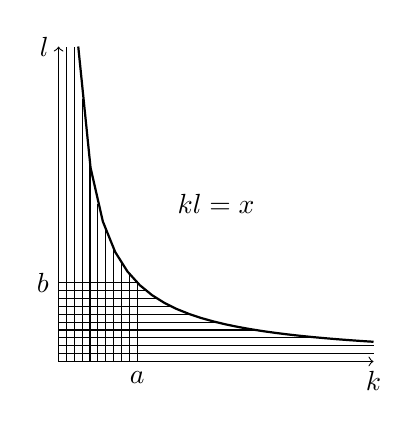
\begin{tikzpicture}
\draw[<->](0,4)--(0,0)--(4,0);
\node[left]at(0,4){$l$};
\node[below]at(4,0){$k$};
\node[left]at(0,1){$b$};
\node[below]at(1,0){$a$};
\node at(2,2){$kl=x$};
\draw[thick,domain=0.25:4] plot(\x,1/\x);
\foreach\x in{0.1,0.2,...,1}\draw(\x,0)--(\x,{min(4,1/\x)});
\foreach\x in{0.1,0.2,...,1}\draw(0,\x)--({min(4,1/\x)},\x);
\end{tikzpicture}
\end{gather*}
We have
\begin{align*}
\abs[\Big]{\frac1x\sum_{k\leq a}\paren[\Big]{\mu(k)\sum_{l\leq x/k}g(l)}} &\leq \frac1x\sum_{k\leq a}\abs[\Big]{\sum_{l\leq x/k}g(l)} \leq \frac1x\sum_{k\leq a}c\sqrt{\frac{x}{k}} \\
&= \frac{c}{\sqrt x}\sum_{k\leq a}\frac{1}{\sqrt k} \\
&= \frac{c}{\sqrt x}\paren[\Big]{2\sqrt a+O(1)}\footnote{by Euler's Sum Formula} \\
&= \frac{c}{\sqrt x}\parenBig{2\sqrt{\frac xb}+O(1)} \\
&= \frac{2c}{\sqrt b} + O\parenBig{\frac1{\sqrt x}} < \epsilon + O\parenBig{\frac1{\sqrt x}}
\end{align*}
where we choose $b$ large enough so $\frac{2c}{\sqrt b}<\epsilon$
\[ \absBig{\frac1x\sum_{l\leq b}g(l)\sum_{k\leq x/l}\mu(k)} \leq \frac1x\sum_{l\leq b}\abs{g(l)}\absBig{\sum_{k\leq x/l}\mu(k)} = \sum_{l\leq b}\frac{\abs{g(l)}}{l}\absBig{\frac{1}{x/l}\sum_{k\leq x/l}\mu(k)} < \epsilon \]
for all $x\geq r$ where $r$ is chosen so that
\[ \frac{\abs{g(l)}}{l} \absBig{\frac{1}{x/l}\sum_{k\leq x/l}\mu(k)} < \frac{\epsilon}{b} \]
for each $l\leq b$ (which we can do by part~(c))
\begin{align*}
\absBig{\frac1x\sum_{k\leq a}\mu(k)\sum_{l\leq b}g(l)} &= \frac1x\absBig{\sum_{k\leq x/b}\mu(k)}\absBig{\sum_{l\leq b}g(l)} \\
&= \frac1b\absBig{\frac1{x/b}\sum_{k\leq x/b}\mu(k)}\cdot c\sqrt b \\
&< \epsilon \text{ for all $x\geq3$}
\end{align*}
where $s$ is chosen large enough.

\textbf{$(3)\implies(4)$} [we have $\frac{\psi(x)}{x}\to1$ we must show $\frac{\vartheta(x)}{x}\to1$] \\
\begin{align*}
\vartheta(x) &= \sum_{p\leq x}\log p \\
\psi(x) &= \sum_{p^k\leq x}\log p = \sum_{p\leq x}\sum_{\substack{k\geq1\\p^k\leq x}}\log p \\
&= \sum_{p\leq x}\log p + \sum_{p\leq x}\sum_{\substack{k\geq2\\p^k\leq x}}\log p \\
&= \vartheta(x) + \sum_{2\leq k\leq\log_2 x}\sum_{p\leq x^{1/k}}\log p \\
&= \vartheta(x) + \sum_{2\leq k\leq\log_2 x}\vartheta(x^{1/k})
\end{align*}
Note that
\[ \vartheta(x) = \sum_{p\leq x}\log p \leq \sum_{p\leq x}\log x \leq x\log x \]
So we have
\begin{align*}
\psi(x)-\vartheta(x) &= \sum_{2\leq k\leq\log_2 x}\vartheta(x^{1/k}) \\
0\leq \psi(x)-\vartheta(x) &\leq \sum_{2\leq k\leq\log_2 x}x^{1/k}\log x^{1/k} \\
&\leq \sum_{2\leq k\leq\log_2 x}x^{1/2}\log x^{1/2} \leq \log_2 x\cdot x^{1/2}\cdot \log x^{1/2} \\
0\leq \frac{\psi(x)}{x}-\frac{\vartheta(x)}{x} &\leq \frac{\log_2 x\cdot\log x^{1/2}}{x^{1/2}} = \frac{(\log x)^2}{2\log 2 \sqrt x} \to 0 \text{ as $x\to\infty$} \\
\therefore\parenBig{\frac{\psi(x)}{x}-\frac{\vartheta(x)}{x}} &\to 0
\end{align*}
and $\frac{\psi(x)}{x}\to1$ so $\frac{\vartheta(x)}{x}\to1$.

\textbf{$(4)\implies(5)$} [we have $\vartheta(x)\sim x$, i.e., $\sum_{p\leq x}\log p\sim x$; we need to show $\pi(x)\sim\frac{x}{\log x}$, i.e., $\sum_{p\leq x}1\sim\frac{x}{\log x}$] \\
We use Abel's Summation Formula with
\[ a(n) = \begin{cases}
\log p & \text{if $n=p$, prime} \\
0 & \text{otherwise}
\end{cases} \]
so $A(x)=\sum_{n\leq x}a(n)=\sum_{p\leq x}\log p=\vartheta(x)$ and $f(t)=\frac{1}{\log t}$ so $f'(t)=\frac{-1}{t(\log t)^2}$ to get
\begin{align*}
\pi(x) &= \sum_{p\leq x}1 = \sum_{n\leq x}a(n)f(n) \\
&= A(x)f(x) - \int_1^x A(t)f'(t)\d t \\
&= \frac{\vartheta(x)}{x} + \int_1^x\frac{\vartheta(t)}{t(\log t)^2}\d t \\
\frac{\pi(x)\log x}{x} &= \frac{\vartheta(x)}{x} + \frac{\log x}{x}\int_1^x\frac{\vartheta(t)}{t(\log t)^2}\d t
\end{align*}
and using l'H\^opital's Rule
\begin{align*}
\lim_{x\to\infty}\frac{\int_1^x\frac{\vartheta(t)\d t}{t(\log t)^2}\footnote{$\to\infty$}}{\frac{x}{\log x}\footnote{$\to\infty$}} %\\
&= \lim_{x\to\infty}\frac{\frac{\vartheta(x)}{x(\log x)^2}}{\frac{\log x-1}{(\log x)^2}} \\
&= \lim_{x\to\infty} \frac{\vartheta(x)/x}{\log x-1} \\
&= 0
\end{align*}
\textbf{$(5)\implies(6)$} [MST $p(n)\sim n\log n$]
\begin{align*}
\lim_{x\to\infty}\frac{\pi(x)\log x}{x} &= 1 \\
\lim_{x\to\infty}(\log\pi(x)+\log\log x-\log x) &= 0 \\
\lim_{x\to\infty}\parenBig{\frac{\log\pi(x)}{\log x}+\frac{\log\log x}{\log x}\footnote{$\to0$}-1} &= 0 \\
\lim_{x\to\infty}\frac{\log\pi(x)}{\log x} &= 1 \\
\therefore \frac{\log\pi(x)}{\log x}\frac{\pi(x)\log x}{x}\footnote{by (5)} &\to 1 \\
\therefore \frac{\pi(x)\log\pi(x)}{x} &\to 1
\end{align*}
Take $x=p(n)$ so $\pi(x)=n$
\[ \frac{n\log n}{p(n)}\to1 . \]
